\chapter{High-Level Design}

\begin{quotation}
"Software development is not a rational process. It's a process made by people with feelings,
with bodies and with thinking. And by putting all those together I can be a more effective
software engineer."
\end{quotation}
\begin{flushright}
Kent Beck
\end{flushright}

A goal without a plan is just a wish. We kickstart this chapter by discussing the workflow model we choose and why it was a good fit for us. We shall then venture into the architectural design of our project and then move towards the functionality of the same.

% ===================================================================================================
% SOFTWARE DEVELOPMENT METHODOLOGY
% ===================================================================================================

\section{Software Development Methodology}
The software development methodology we have used is Xtreme Programming from the family of Agile Processes.

As Roger S. Pressman notes in his book \textit{Software Engineering: A Practioner's Approach}

\begin{quotation}
"[Agile processes] are appropriate for many types of project and are particularly useful when web applications are engineered."
\end{quotation}

We will first give you an account as to what XP is and then justify our choice of workflow.

\begin{figure}
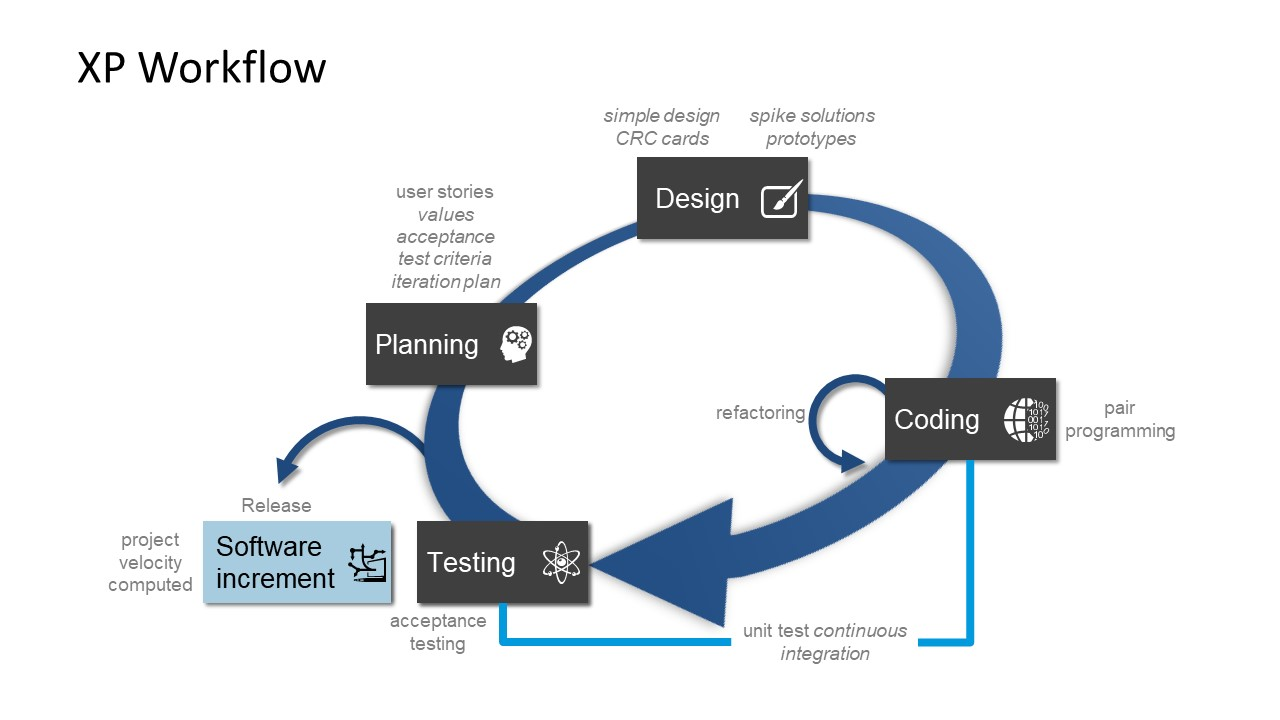
\includegraphics[scale=0.5]{images/xtreme.jpg}
\caption{}
\label{fig:xtreme}
\end{figure}

\subsection{What is it?}

Extreme programming (XP) Figure ~\ref{fig:xtreme}, is a software development methodology which is intended to improve software quality and responsiveness to changing customer requirements. As a type of agile software development, it advocates frequent "releases" in short development cycles, which is intended to improve productivity and introduce checkpoints at which new customer requirements can be adopted.

Other elements of extreme programming include: programming in pairs or doing extensive code review, unit testing of all code, avoiding programming of features until they are actually needed, a flat management structure, code simplicity, and clarity, expecting changes in the customer's requirements as time passes and the problem is better understood, and frequent communication with the customer and among programmers.

This methodology takes its name from the idea that the beneficial elements of traditional software engineering practices are taken to "extreme" levels. As an example, code reviews are considered a beneficial practice; taken to the extreme, the code can be reviewed continuously, i.e. the practice of pair programming.

\subsection{Why we chose it?}

Developing any software on web platform entails change as its introductory name. Clearly, owing to its just-in-time functionality, web development requires that the developers be constantly looking out for change and bring it into the platform as soon as possible. This intrinsic nature of web-development prompted us to undertake a process model that would naturally lend itself to rapid change and fast build. And thus we choose XP as an obvious model that meets our requirements adequately.

\section{Architecture}

\begin{center}
\begin{figure}[h!]
    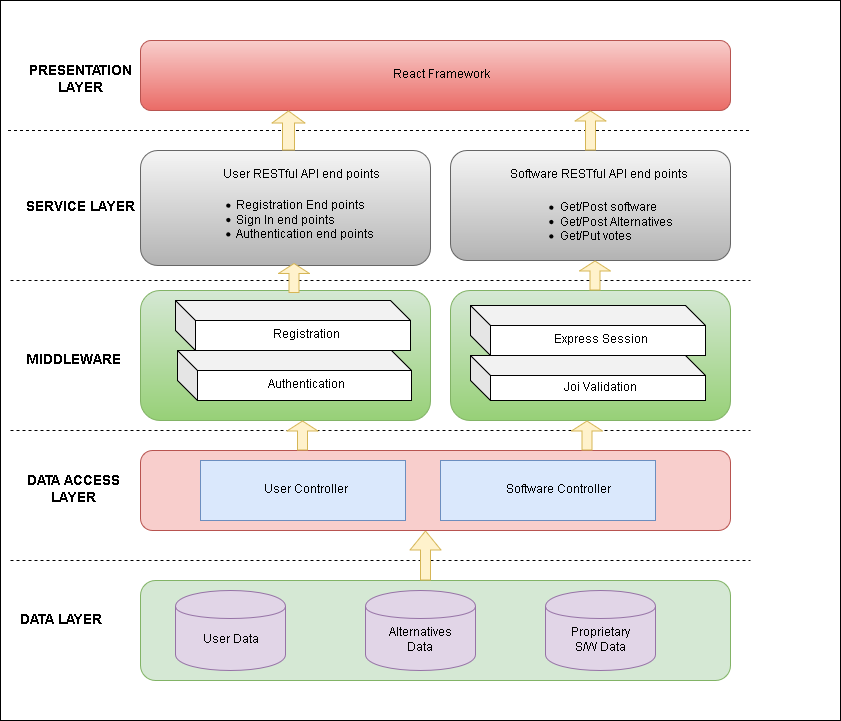
\includegraphics[scale=0.5]{images/architecture.png}
    \caption{Architectural diagram for AlterFOSS}
    \label{fig:architecture}
\end{figure}
\end{center}


As the architecture shows, the application works in five different layers - Data layer, data access layer, middleware, service layer and presentation layer. The explaination of each of these layers is as follows:

\begin{itemize}
\item \textbf{Data Layer}: This layer will deal with the data source, i.e the database which is used to store all the data necessary for this application to function. This is the MongoDB database in our case, which is a free and NoSQL database. The data to be stored is the user data and the data related to the softwares and their alternatives.

\item \textbf{Data Access Layer}: This layer will deal with accessing the data that is stored in the database and changing it to a format which can be used by the application for further processing, such as creating objects out of the documents stored in the MongoDB database. This layer will comprise of modules consisting of functions to deal with both the user data and the software data stored at the data layer.

\item \textbf{Middleware}: This layer consists of middleware which deals with add-on tasks such as input validation, session handling using express, user authentication and registration. Various other minor middlewares are also used throughout the project which aid in integration of the data access layer with the service layer.

\item \textbf{Service layer}: This layer is the one responsible for getting the validated data through RESTful api end points and presenting it to the user on the front end as well as take the input from user, send it to the middleware for further validation before storing it in the database. Basically, this layer is used to glue together the front-end to the back-end.

\item \textbf{Presentation layer}: This layer is the one which will be directly accessible to the user and the point via which the user interacts with the application. It is designed using the React Framework and consists of various forms, fields, tables  and components to enable the user to perform various actions like searching, posting data, retrieving data, voting et cetera which enable the smooth functioning of the application.

\end{itemize}
    
% ===================================================================================================
% FUNCTIONAL SPECIFICATIONS SECTION
% ===================================================================================================
\section{Functional Specifications}
This section deals with various functional components of the application and their associated purpose.

\subsection{Search Softwares}
Name of module: searchProprietarySoftware
Parameters: Text entered by the user at the front end
Purpose: This functional component will be used to search for proprietary softwares that 
have already been requested by some user to get its alternatives.

\subsection{Request for alternatives for a software}

Name of module: addProprietarySoftwares
Parameters: The name of the software for which alternatives are desired, tags defining the software.
Purpose: This functional component is used when a user wants to request for alternatives to proprietary software that is not already available on the platform. The user will need to specify the name of the software along with the tags to categorize the software, which can be later used to fetch the alternatives.

\subsection{Suggest alternatives}

Name of module: addAlternatives
Parameters: The name of the alternative software along with the handle which uniquely categorizes the software 
Purpose: This functional component is used when the user wishes to add new alternative software to the 

\subsection{Check license of a software}

Name of module: checkLicense
Parameters: Name of the software for which the license is to be checked
Purpose: This functional component will be used to show the license under which the software is published. The user can also get more detailed information about the license via this module. The license for the software will be specified by the user who suggested the alternative.

\subsection{Upvote/Downvote a particular alternative}

Name of module: upVote/downVote
Parameters: A unique identifier for the software which will be picked up by the front end during the user's interaction with the voting feature
Purpose: This functional component is utilized when the user wishes to upvote or downvote a software 

\subsection{Signup/Login/Authenticate}

Name of module: authenticate/register
Parameters: The required user credentials depending on the operation to be performed
Purpose: Used to start a session by either logging in the user or creating a new user in case the corresponding entry for the user does not exist. This module will also authenticate the user in case he wishes to login by checking the user-id and password. For security reasons, the password hash is stored rather than the password in clear text.




